\documentclass[a4paper, 11pt]{article}
\usepackage{comment} % enables the use of multi-line comments (\ifx \fi) 
\usepackage{fullpage} % changes the margin
\usepackage{amsmath}
\usepackage{graphicx}


\begin{document}


\noindent
\LARGE\textbf{The Photoelectric Effect} \\
\\
\normalsize \textbf{By: Kevin Dang}



\section*{Introduction}

The objective of this experiment was to investigate the photoelectric effect, where we used Einstein's equation to obtain Planck's constant and the cutoff frequency. The experiment involved collecting data points on stopping voltage, determining whether photoelectron emission is related to intensity of light, and looking at the time response of photocurrent. \\
\\
Some equations relevant to this experiment include:

Energy: $E = hf$

Einstein's equation: $eV_{stop} = hf - E_0$

Linear: $V_{stop} = \frac{h}{e}f - \frac{h}{e}f_0$

Electron Power: $P_e = P_{LED}\frac{A_{e}}{A_{PC}}$


\section*{Equipment}

\begin{itemize}
\item Phototube
\item Potentiometer
\item Power supply
\item 2 multimeters (used as voltmeters)
\item 8 Light emitting diodes from 390nm to 935nm
\item Variable intensity LED
\item Oscillator driven LED
\item Oscilloscope
\item Wave generator
\end{itemize}	


\section*{Experimental Procedure}

\subsubsection*{Stopping Voltage}
\begin{enumerate}
\item Arranged the equipment as shown in Figure 2 of the photoelectric effect lab guide.
\item Placed an LED into the power supply, and turned on the power. Aligned the LED with the phototube, and turned off nearby light sources.
\item Set photocurrent to zero while keeping the potentiometer on and measured the stopping voltage of the LED.
\item Repeated the above steps for 8 LEDs.
\end{enumerate}

\subsubsection*{Light Intensity Effect}
\begin{enumerate}
\item Placed the variable intensity LED into the power supply, and turned on the power. Aligned the LED with the phototube, and turned off nearby light sources.
\item Set photocurrent to zero while keeping the potentiometer on and measured the stopping voltage of the LED.
\item Turned off potentiometer to measure photocurrent. Photocurrent was measured independently of stopping voltage, so there were two separate datasets.
\item Repeated above steps for the 4 light intensity levels using one variable intensity LED.
\end{enumerate}

\subsubsection*{Photocurrent Time Response}
\begin{enumerate}
\item Connected phototube to channel 1 of the oscilloscope, using an adaptor and connected wave generator to channel 2 of the oscilloscope and to the oscillator-driven LED.
\item Adjusted oscilloscope and wave generator appropriately to see one period of oscillation.
\item Recorded the time constant after measuring photocurrent as a function of time.
\end{enumerate}


\section*{Results}

\subsubsection*{Stopping Voltage}

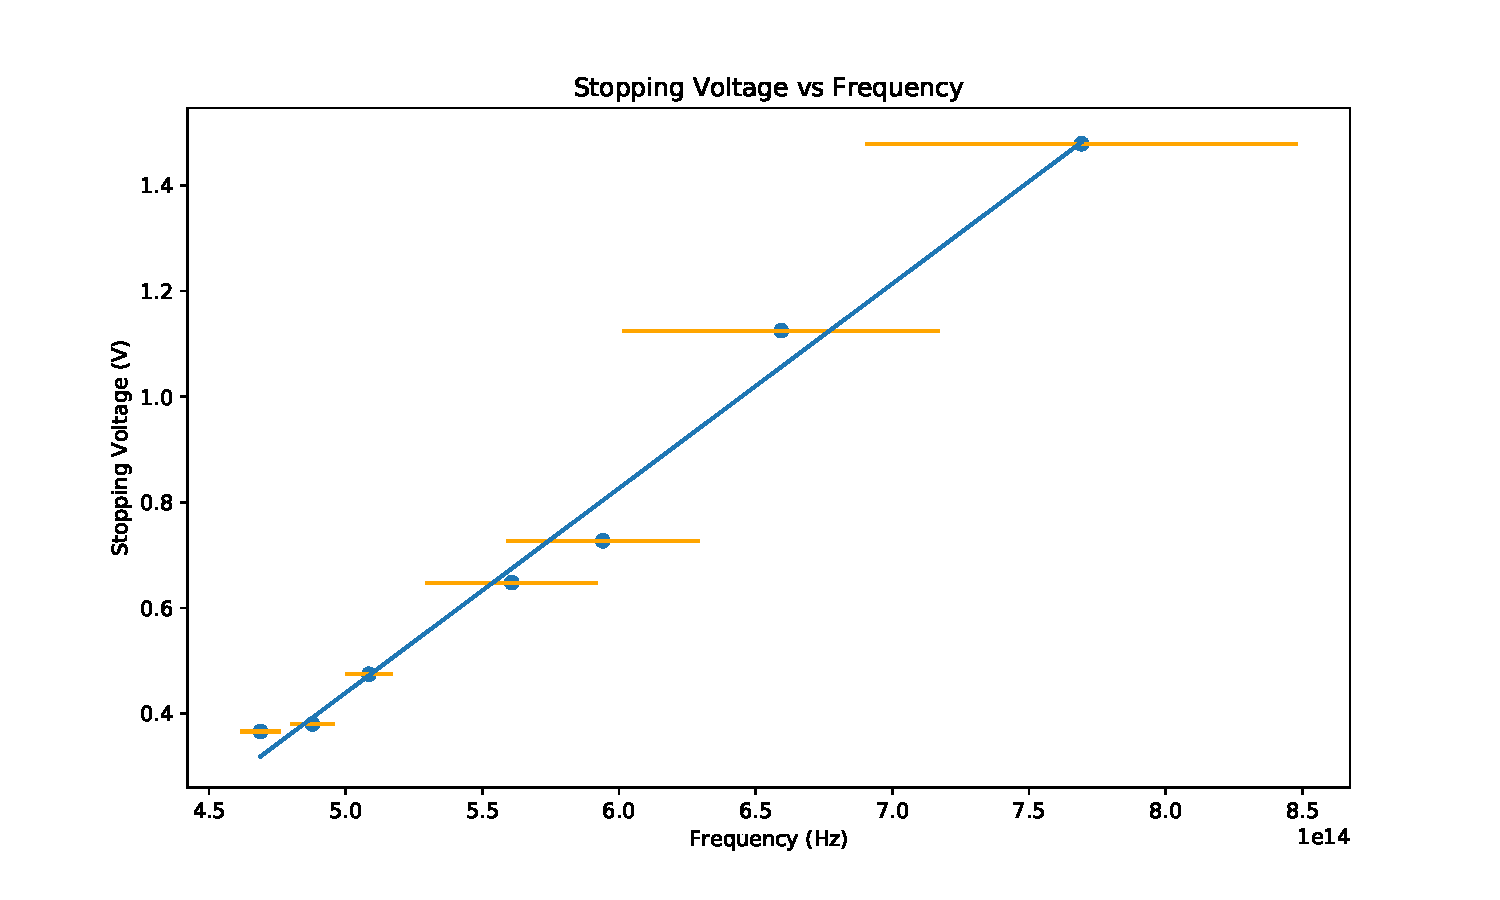
\includegraphics[width=\textwidth]{vstop_freq.pdf}
Linear equation: $V_{stop} = (3.872 \times 10^{-15}) \times frequency - 1.497$ \\
Reduced chi-squared: $\chi^{2}_{red} = 10970$ \\
\\
The model fit is poor due to large, varying errors as seen in the plot. These errors were given in the Photoelectric effect lab guide.
\\
Planck's constant ($h$): We have the slope of the line, which represents Planck's constant divided by the charge of an electron ($e = 1.602 \times 10^{-19} C$).
\begin{center}
$\frac{h}{e} = 3.872 \times 10^{-15} \Rightarrow h = (3.872 \times 10^{-15})(1.602 \times 10^{-19})$ 
\\
$h = 6.203 \times 10^{-34} \pm (0.320 \times 10^{-34}) \frac{kg \cdot m^2}{s}$
\end{center}
The literature value for Planck's constant is $6.626 \times 10^{-34}$, so our calculated value has an error of approximately 6\%. The literature value is slightly outside the range of uncertainty, which shows that our results were not very accurate or our errors were rather small.\\
\\
Cutoff frequency ($f_0$): The intercept of the line represents $-\frac{h}{e}f_0$, as part of the linear equation given in the introduction.
\begin{center}
$-\frac{h}{e}f_0 = -1.497 \Rightarrow f_0 = \frac{(1.497)(1.602 \times 10^{-19})}{6.203 \times 10^{-34}} = 3.865 \times 10^{14} \pm (0.363 \times 10^{14}) Hz$
\end{center}
In collecting our data, we were unable to obtain a voltage measurement for the infrared LED, which had a wavelength of 935nm. Let us convert the wavelength to a frequency:
\begin{center}
$f = \frac{c}{\lambda} = \frac{3 \times 10^{8}}{935 \times 10^{-9}} = 3.209 \times 10^{14}Hz$
\end{center}
This calculation shows that the infrared LED had a frequency below the cutoff frequency, hence we were not able to detect the voltage for the infrared LED. \\
\\
Work function ($E_0$): This can be calculated by the energy equation. 
\begin{center}
$E_0 = hf_0 = (6.203 \times 10^{-34})(3.865 \times 10^{14}) = 2.398 \times 10^{-19} \pm (0.349 \times 10^{-19}) J$
\end{center}

\subsubsection*{Light Intensity Effect}

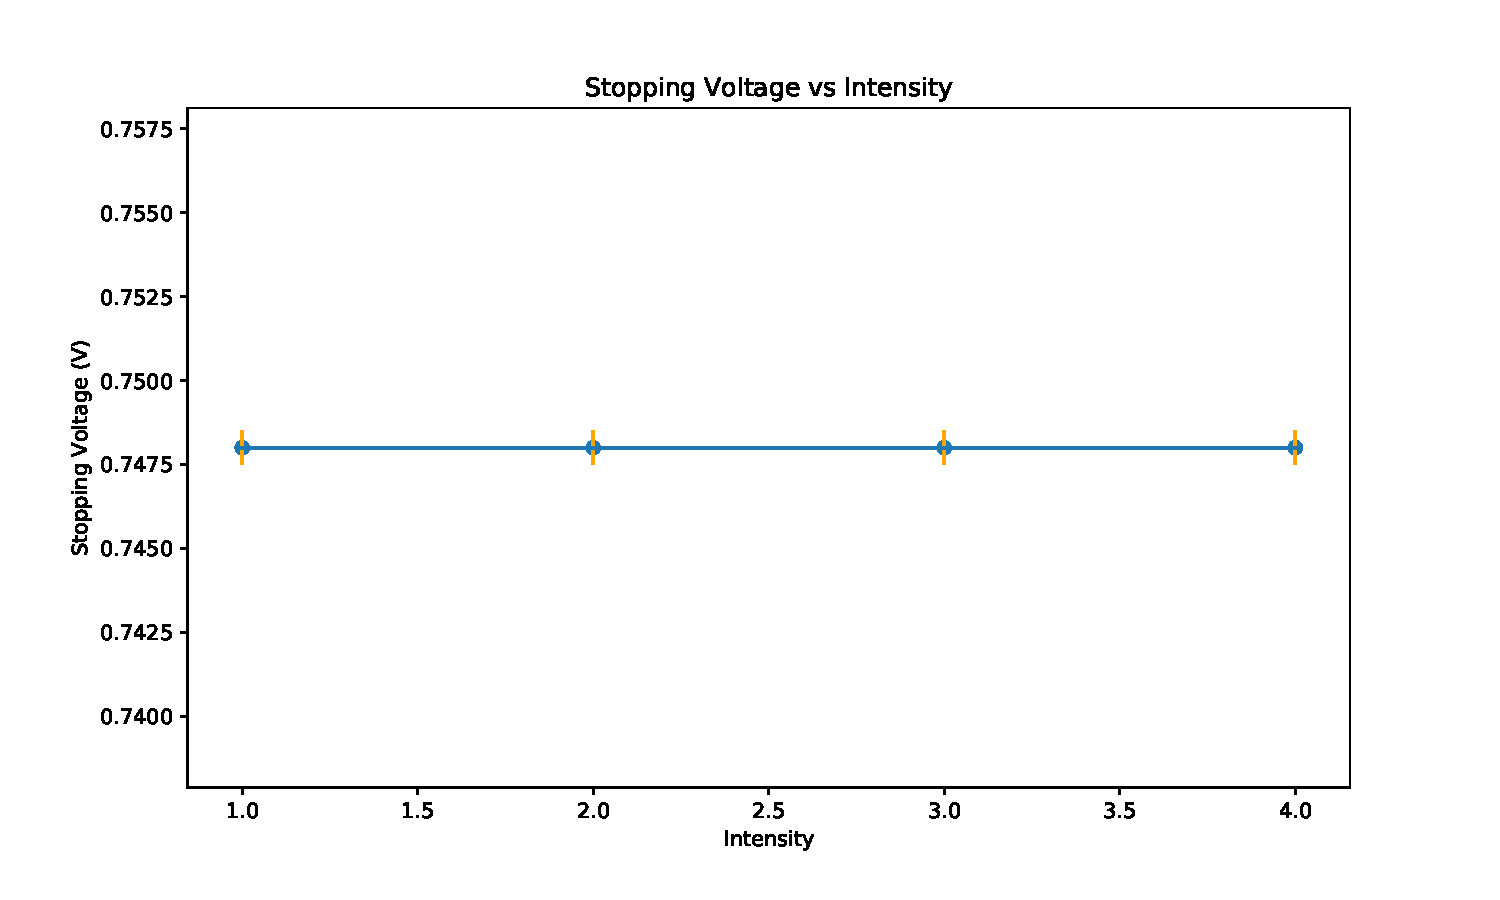
\includegraphics[width=\textwidth]{vstop_inten.pdf}
Linear equation: $V_{stop} = (-2.181 \times 10^{-12}) \times Intensity + 0.748$ \\
Reduced chi-squared: $\chi^{2}_{red} = 4.756 \times 10^{-17}$ \\
\\
From the linear equation we can see that the slope is almost zero, which means that the stopping voltage remains constant across varying intensities. The reduced chi-squared value is extremely small which suggests overfitting, however this can be explained by the small number of data points, and very small errors. The results indicate that the stopping voltage does not depend on intensity.

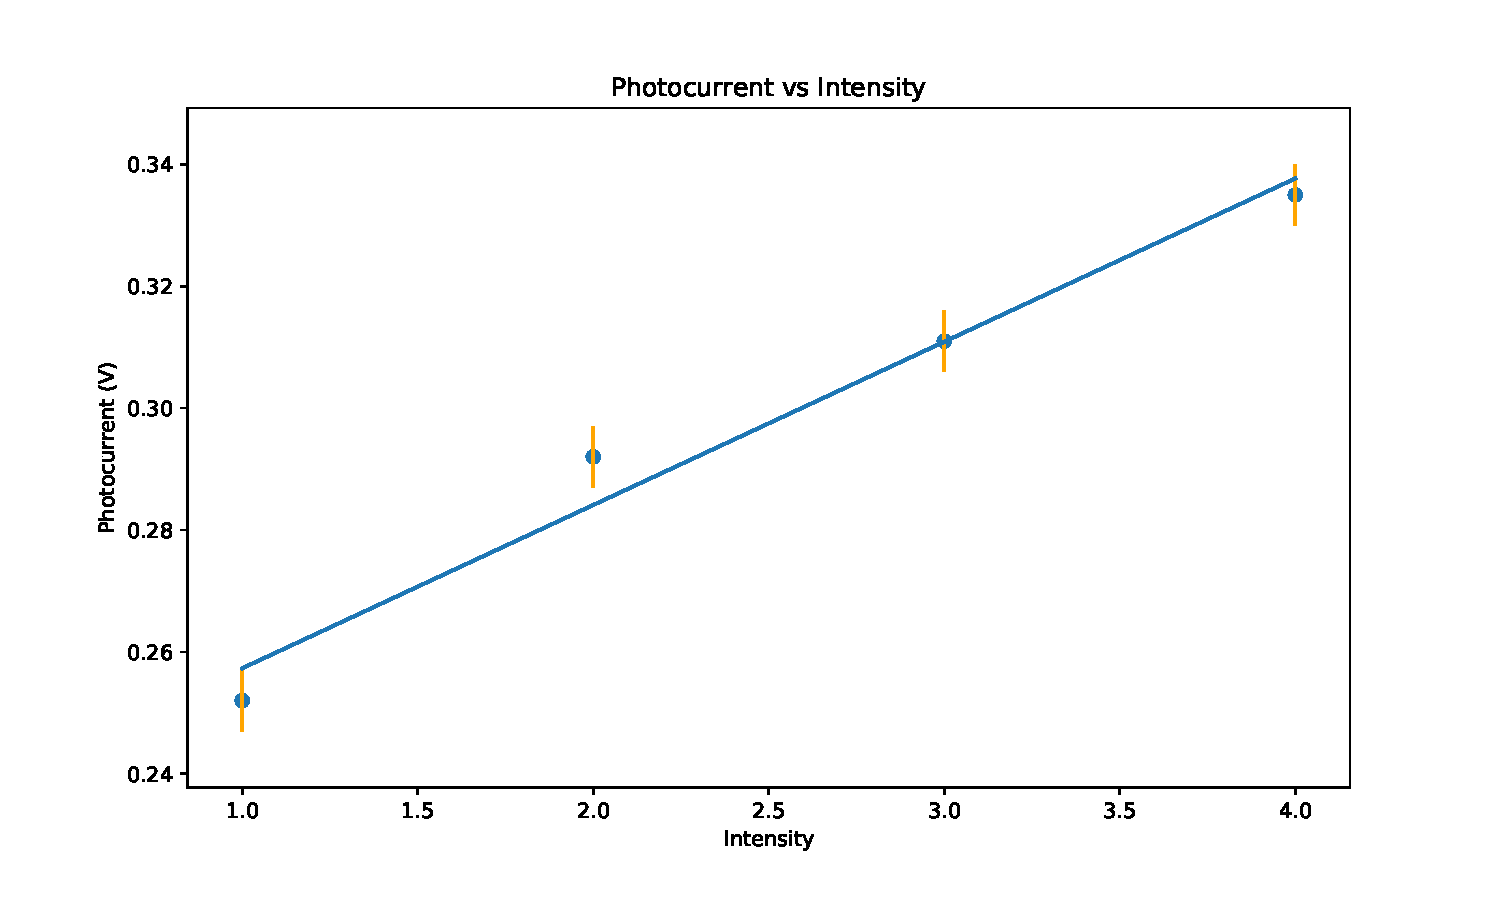
\includegraphics[width=\textwidth]{photo_inten.pdf}
Linear equation: $Photocurrent = 0.0268 \times Intensity + 0.230$ \\
Reduced chi-squared: $\chi^{2}_{red} = 1.956$ \\
\\
The above results show that photocurrent varies with intensity.

\subsubsection*{Photocurrent Time Response}
Using the oscilloscope and wave generator, we estimated the time constant to be $200 \pm 10\mu s$, or $0.0002 \pm 0.00001 s$.

To calculate energy absorbed by each electron in a second (also known as power), we use the following equation:
\begin{center}
$P_e = P_{LED}\frac{A_{e}}{A_{PC}} = 0.060 \frac{\pi(0.15 \times 10^{-9})^2}{3.23 \times 10^{-5}} = 1.313 \times 10^{-17} \frac{J}{s}$
\end{center}
Building on this calculation, we can estimate the time needed by an electron to escape the photocathode after absorbing enough energy:
\begin{center}
$t_{escape} = \frac{E_0}{P_e} = \frac{2.398 \times 10^{-19}}{1.313 \times 10^{-17}} = 0.0183s$
\end{center}
The calculated escape time is significantly larger then the experimental time constant. This suggests that absorption of light is much faster in reality.

\section*{Conclusion}
The stopping voltage is a linear function of frequency, and this relationship was used to determine the experimental values for Planck's constant, the cutoff frequency, and the work function. We obtained a value of $ h = 6.203 \times 10^{-34} \frac{kg \cdot m^2}{s}$, which is a bit small compared to the literature value. The cutoff frequency was $3.865 \times 10^{14} Hz$, which explains why were not able to obtain a voltage reading for the infrared light whose frequency of $3.209 \times 10^{14} Hz$ was below the cutoff. The value for the work function was $2.398 \times 10^{-19}$.

Looking at the light intensity effect, we obtained results which showed that the stopping voltage does not depend on light intensity, while there appeared to be a linear relationship between photocurrent and intensity.

Using the oscilloscope, we estimated the time constant to be about 0.0002 seconds. We also calculated the energy absorbed by an electron in a second by using the fact that electrons have a radius of about $0.15nm$, and we were given values for the electric power and photocathode area. Taking this value, and the value for the work function calculated earlier, we obtained a final result for the escape time, which was 0.0183 seconds. This time is slower than the experimental time constant, which shows that the absorption of light is much faster in reality, and confirms the quantum theory.


\end{document}
